\documentclass[hyperref={pdfpagelabels=false}]{beamer}
\usepackage[ngerman]{babel}
\usepackage[utf8]{inputenc}


%\usepackage{lmodern}

\title{Thema 2.3: Apache Spark}   
\subtitle{Skalierbare verteilte Datenanalyse}
\author{Lukas Wappler} 
\date{\today} 

\usetheme{Malmoe}

\usepackage{beamerthemeshadow}


\useoutertheme{infolines}

%  \beamersetuncovermixins{\opaqueness<1>{25}}{\opaqueness<2->{15}}
%  sorgt dafuer das die Elemente die erst noch (zukuenftig) kommen 
%  nur schwach angedeutet erscheinen 
\beamersetuncovermixins{\opaqueness<1>{25}}{\opaqueness<2->{15}}
% klappt auch bei Tabellen, wenn teTeX verwendet wird\ldots



%NO FOOTLINE
%gets rid of bottom navigation bars
%\setbeamertemplate{footline}[frame number]{}

%gets rid of bottom navigation symbols
\setbeamertemplate{navigation symbols}{}

%gets rid of footer
%will override 'frame number' instruction above
%comment out to revert to previous/default definitions
\setbeamertemplate{footline}{}


%\setbeamertemplate{frametitle}{\nointerlineskip  
 %   \begin{beamercolorbox}[wd=\paperwidth,ht=2.75ex,dp=1.375ex]{frametitle}
  %      \hspace*{2ex}\insertframetitle \hfill {\insertframenumber} \hspace*{1ex}%
   % \end{beamercolorbox}}

%\addtobeamertemplate{headline}{}{\rule{\paperwidth}{3pt}}

\addtobeamertemplate{headline} 
{
  \leavevmode%
  \hbox{%
  \begin{beamercolorbox}[wd=.333333\paperwidth,ht=2.25ex,dp=1ex,center]{author in head/foot}%
    Lukas Wappler
		%\usebeamerfont{author in head/foot}\insertsection
  \end{beamercolorbox}%
  \begin{beamercolorbox}[wd=.333333\paperwidth,ht=2.25ex,dp=1ex,center]{title in head/foot}%
   
		Thema 2.3: Apache Spark		
  \end{beamercolorbox}%
  \begin{beamercolorbox}[wd=.333333\paperwidth,ht=2.25ex,dp=1ex,right]{date in head/foot}%
    \usebeamerfont{date in head/foot}\insertshortdate{}\hspace*{2em}
    \insertframenumber{} / \inserttotalframenumber \hspace*{2ex} 
  \end{beamercolorbox}}%
  \vskip0pt%
}


\begin{document}




\begin{frame}[plain,noframenumbering]
\titlepage
\end{frame} 


\begin{frame}
\frametitle{Inhaltsverzeichnis}
\setcounter{tocdepth}{1}
\tableofcontents
\end{frame} 





\section{} 
\begin{frame}
\frametitle{} 
\begin{center}
\textit{\LARGE{”Statistical thinking will one day be as necessary for efficient citizenship
as the ability to read and write.“}}
\end{center}

\begin{flushright}
\footnotesize{H.G. WELLS (1866-1946)\\ Science-Fiction-Roman-Autor\\ Der Krieg der Welten}
\end{flushright}

\end{frame}


\section{Einleitung} 
\begin{frame}
\frametitle{Einleitung} 

Heutige Probleme:
\begin{itemize}
\item  Immer mehr Daten 
\item  Datenanalysen müssen immer schneller werden
\item  Keine teuren Supercomputer nutzen
\end{itemize}  

\huge{Ist Apache Spark die Lösung?}


\end{frame}

\section{Apache Spark} 
\begin{frame}
\frametitle{Apache Spark} 


\begin{itemize}
	\item 2009 im AMPLab ins Leben gerufen
	\item 2013 von der Apache Software Foundation übernommen
	\item 2014 Top Level Projekt	
	\item OpenSource	
\end{itemize}

\end{frame}

\subsection{Kern-Bibliotheken / Komponenten}
\begin{frame} 
\frametitle{Kern-Bibliotheken / Komponenten}



\begin{figure}[h]
  \centering
  \fbox{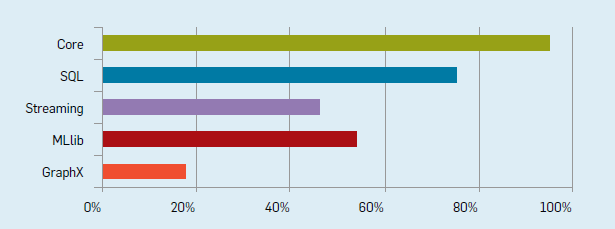
\includegraphics[width=100mm]{../../seminararbeit/bilder/spark_komponenten_nutzung.png}}	  
\end{figure}



\end{frame}

\subsubsection{Spark-Core}
\begin{frame} 
\frametitle{Spark-Core}

%\begin{itemize}
	%\item SparkContext
	%\item Cluster Manager
	%\item Worker Nodes		
%\end{itemize}

\begin{figure}[h]
  \centering
  \fbox{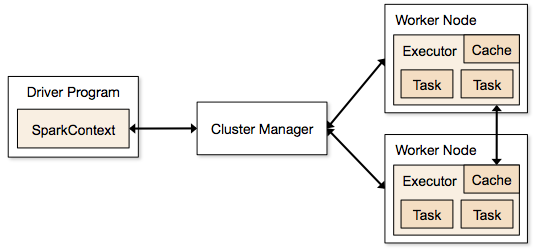
\includegraphics[width=80mm]{../../seminararbeit/bilder/cluster-overview.png}}
\end{figure}

\end{frame}

\subsubsection{RDD’s}
\begin{frame} 
\frametitle{RDD’s}

\begin{itemize}
	\item belastbare (fehlertollerant / ausfallsicher)
	\item verteilt (Daten lassen sich aufteilen)
	\item nach Erstellung nur lesbar
\end{itemize}

\end{frame}


\subsection{SQL-Abfragen}
\subsubsection{Spark-SQL}
\begin{frame} 
\frametitle{Spark-SQL \& Dataframes}
\begin{itemize}
	\item Eine Verbesserung von Shark
	\item kombiniert prozedurale Abfragen \& relationale Datenbankabfragen
	\item Neben RDD's werden auch DataFrames verwendet.
	\item Anbindung unterschiedlichster Datenquellen
\end{itemize}
\end{frame}


\subsection{Verarbeitung von Datenströmen (Spark-Streaming)}
\begin{frame} 
\frametitle{Verarbeitung von Datenströmen (Spark-Streaming)}

\begin{itemize}
	\item RDD's werden zu DStreams erweitert
	\item DStreams verwalten RDD's
\end{itemize}

\begin{figure}[h]
  \centering
  \fbox{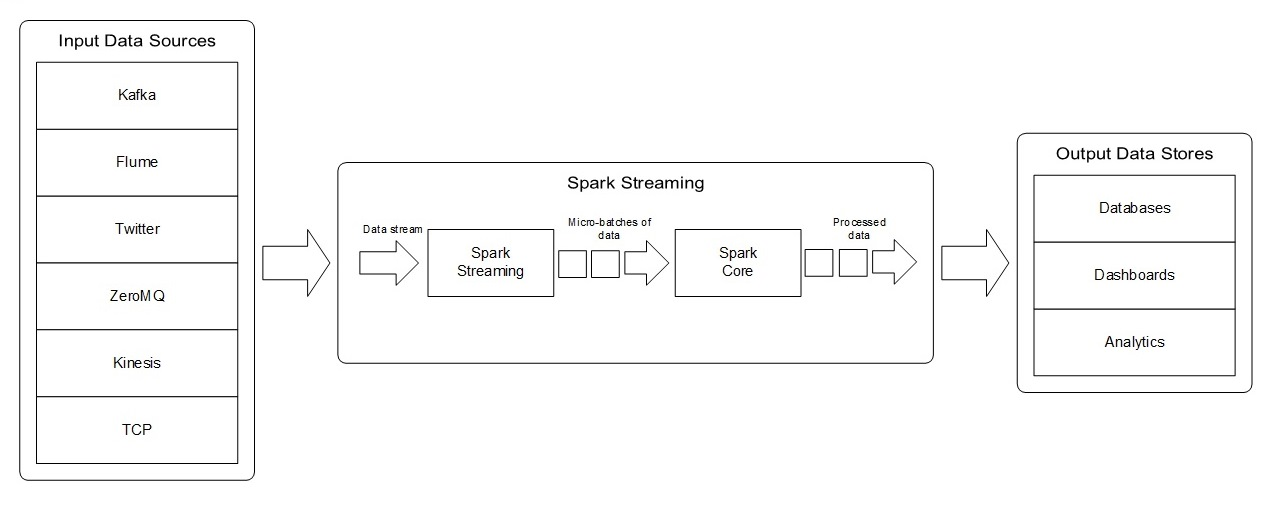
\includegraphics[width=110mm]{../../seminararbeit/bilder/spark_streaming.jpg}}
\end{figure}

\end{frame}


\subsection{Berechnungen auf Graphen (GraphX)}
\begin{frame} 
\frametitle{Berechnungen auf Graphen (GraphX)}

\begin{itemize}
	\item Property-Graphen
	\item Abbildung in RDD-Tupeln
	\item 1. RDD enthält Ecken
	\item 2. RDD enthält Kanten	
\end{itemize}

\begin{figure}[h]
  \centering
  \fbox{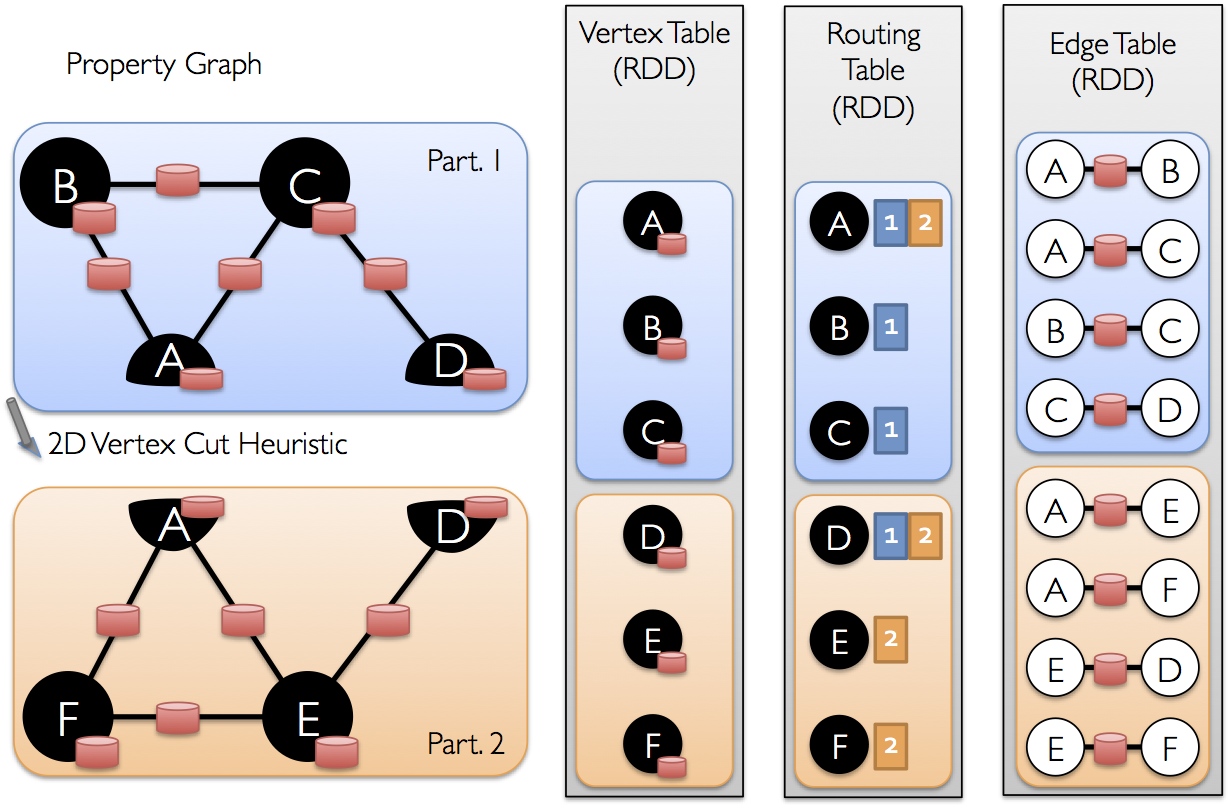
\includegraphics[width=80mm]{../../seminararbeit/bilder/vertex_routing_edge_tables.png}}
\end{figure}

\end{frame}

\subsection{Maschinelles Lernen (MLlib)}
\begin{frame} 
\frametitle{Maschinelles Lernen (MLlib)}

\begin{itemize}
	\item Nutzt DataFrames
	\item Transformator
	\item Estimator
	\item Pipeline
\end{itemize}

\begin{figure}[h]
  \centering
  \fbox{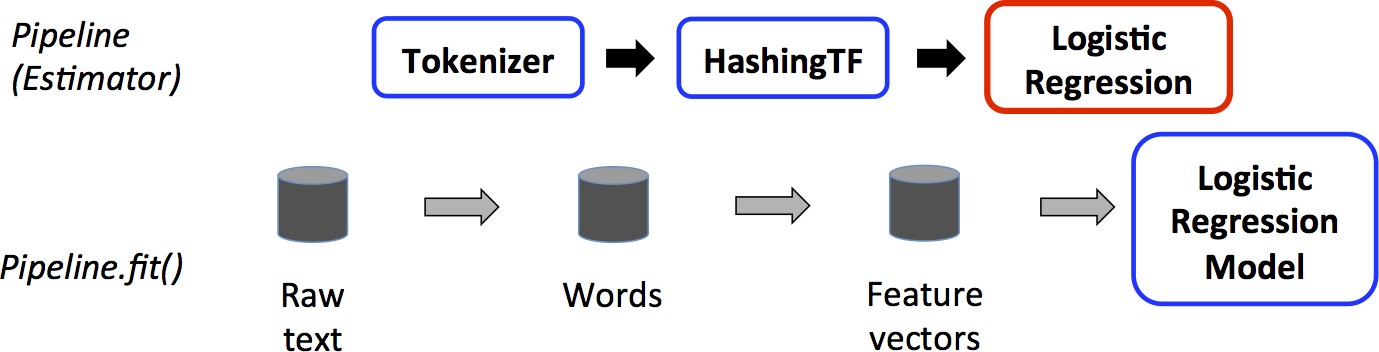
\includegraphics[width=110mm]{../../seminararbeit/bilder/ml-pipeline.png}}
\end{figure}

\end{frame}

\subsection{Skalierung von R Programmen (SparkR)}
\begin{frame} 
\frametitle{Skalierung von R Programmen (SparkR)}

\begin{itemize}
	\item R läuft nur in einem Thread
	\item R-JVM Brücke von R zu Java
	\item Kommunikation über Sockets 
\end{itemize}
\begin{figure}[h]
  \centering
  \fbox{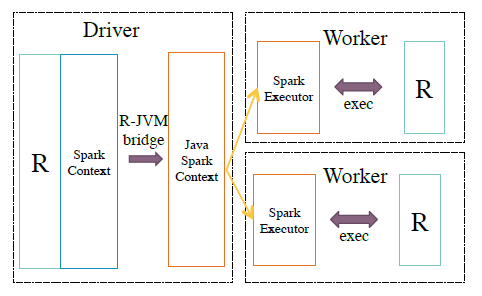
\includegraphics[width=70mm]{../../seminararbeit/bilder/spark_r_architecture.PNG}}
\end{figure}

\end{frame}



\section{Mehrere Komponenten im Verbund}
\begin{frame} 
\frametitle{Mehrere Komponenten im Verbund}

SparkCore, SparkSQL und MLlib im Verbund: 
\begin{itemize}	
	\item 100.000 Mitarbeiter Datensätze
	\item JSON-einlesen	
	\item Suchbegriffe trainieren
	\item Vorhersagen treffen
	\item Daten reduzieren	
	\item Sortieren
	\item Ausgabe der Ergebnisse	
\end{itemize}

\end{frame}


\section{Mehrere Komponenten im Verbund}
\begin{frame} 
\frametitle{Mehrere Komponenten im Verbund}

Demo: Live oder Video.

\end{frame}


\section{Performance}
\begin{frame} 
\frametitle{Performance}

\begin{itemize}
	\item schwer zu messen
	\item Fehler sind schwer zu lokalisieren
	\item Seiteneffekte bei verteilen Operationen	
\end{itemize}

\end{frame}

 \subsection{Besonderheiten bei der Speichernutzung}
\begin{frame} 
\frametitle{Besonderheiten bei der Speichernutzung}

\begin{itemize}
	\item Nutzung des Arbeitsspeichers
	\item speicherplatzeffiziente Datenstrukturen
	\item komprimierte Daten können Blockgrößen überschreiten	
\end{itemize}

\end{frame}

 \subsection{Netzwerk und I/O-Traffic}
\begin{frame} 
\frametitle{Netzwerk und I/O-Traffic}

\begin{itemize}
	\item Zero-copy I/O
	\item Off-heap network buffer management
	\item mehrere Verbindungen	
\end{itemize}

\end{frame}


\section{Nutzung und Verbreitung}
\begin{frame} 
\frametitle{Nutzung und Verbreitung}

\begin{itemize}
	\item Skala, Python, Java, (R)
	\item viele Datenquellen
	\item viele Dateiformate	
	\item über 400 contributors
	\item aus über 100 Unternehmen
	\item Konferenzen (Spark Summit)
	\item 12,779 Sterne (Github)
\end{itemize}

\begin{figure}[h]
  \centering
  \fbox{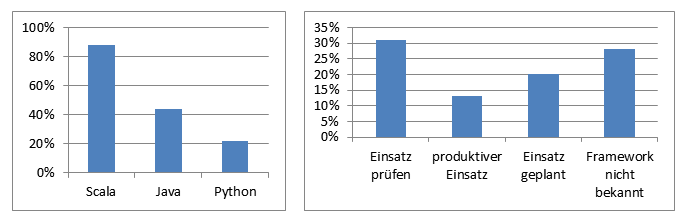
\includegraphics[width=100mm]{../../seminararbeit/excel/Nutzung.png}}
\end{figure}

\end{frame}


\section{ Fazit}
\begin{frame} 
\frametitle{}

\begin{itemize}
	\item vielfältig einsetzbar
	\item kann mit Speziallösungen mithalten
	\item gute Dokumentation \& Literatur
	\item Mischung verschiedener Datenstrukturen schwierig
	\item veraltete News, Blogs oder Foren
	\item kostengünstig
	\item flexibel
\end{itemize}

\end{frame}

\section{Ausblick und Weiterentwicklung}
\begin{frame} 
\frametitle{Ausblick und Weiterentwicklung}

\begin{itemize}
	\item ständige Weiterentwicklung
	\item Code ist über Github verfügbar
	\item 51 Releases (bzw. RC's)
	\item über 19 commits
	\item immer wieder Performancesteigerungen
\end{itemize}

\end{frame}


\section{Vielen Dank}
\begin{frame} 
\frametitle{Vielen Dank}

\begin{center}
\Huge{Vielen Dank für Ihre Aufmerksamkeit!}
\end{center}

\end{frame}


\end{document}